Il layer di \textit{presentation} di Mole.io � rappresentato da mole-suit.

Il server mole-suit � realizzato in Node.js e 

\begin{figure}[h]
\centering
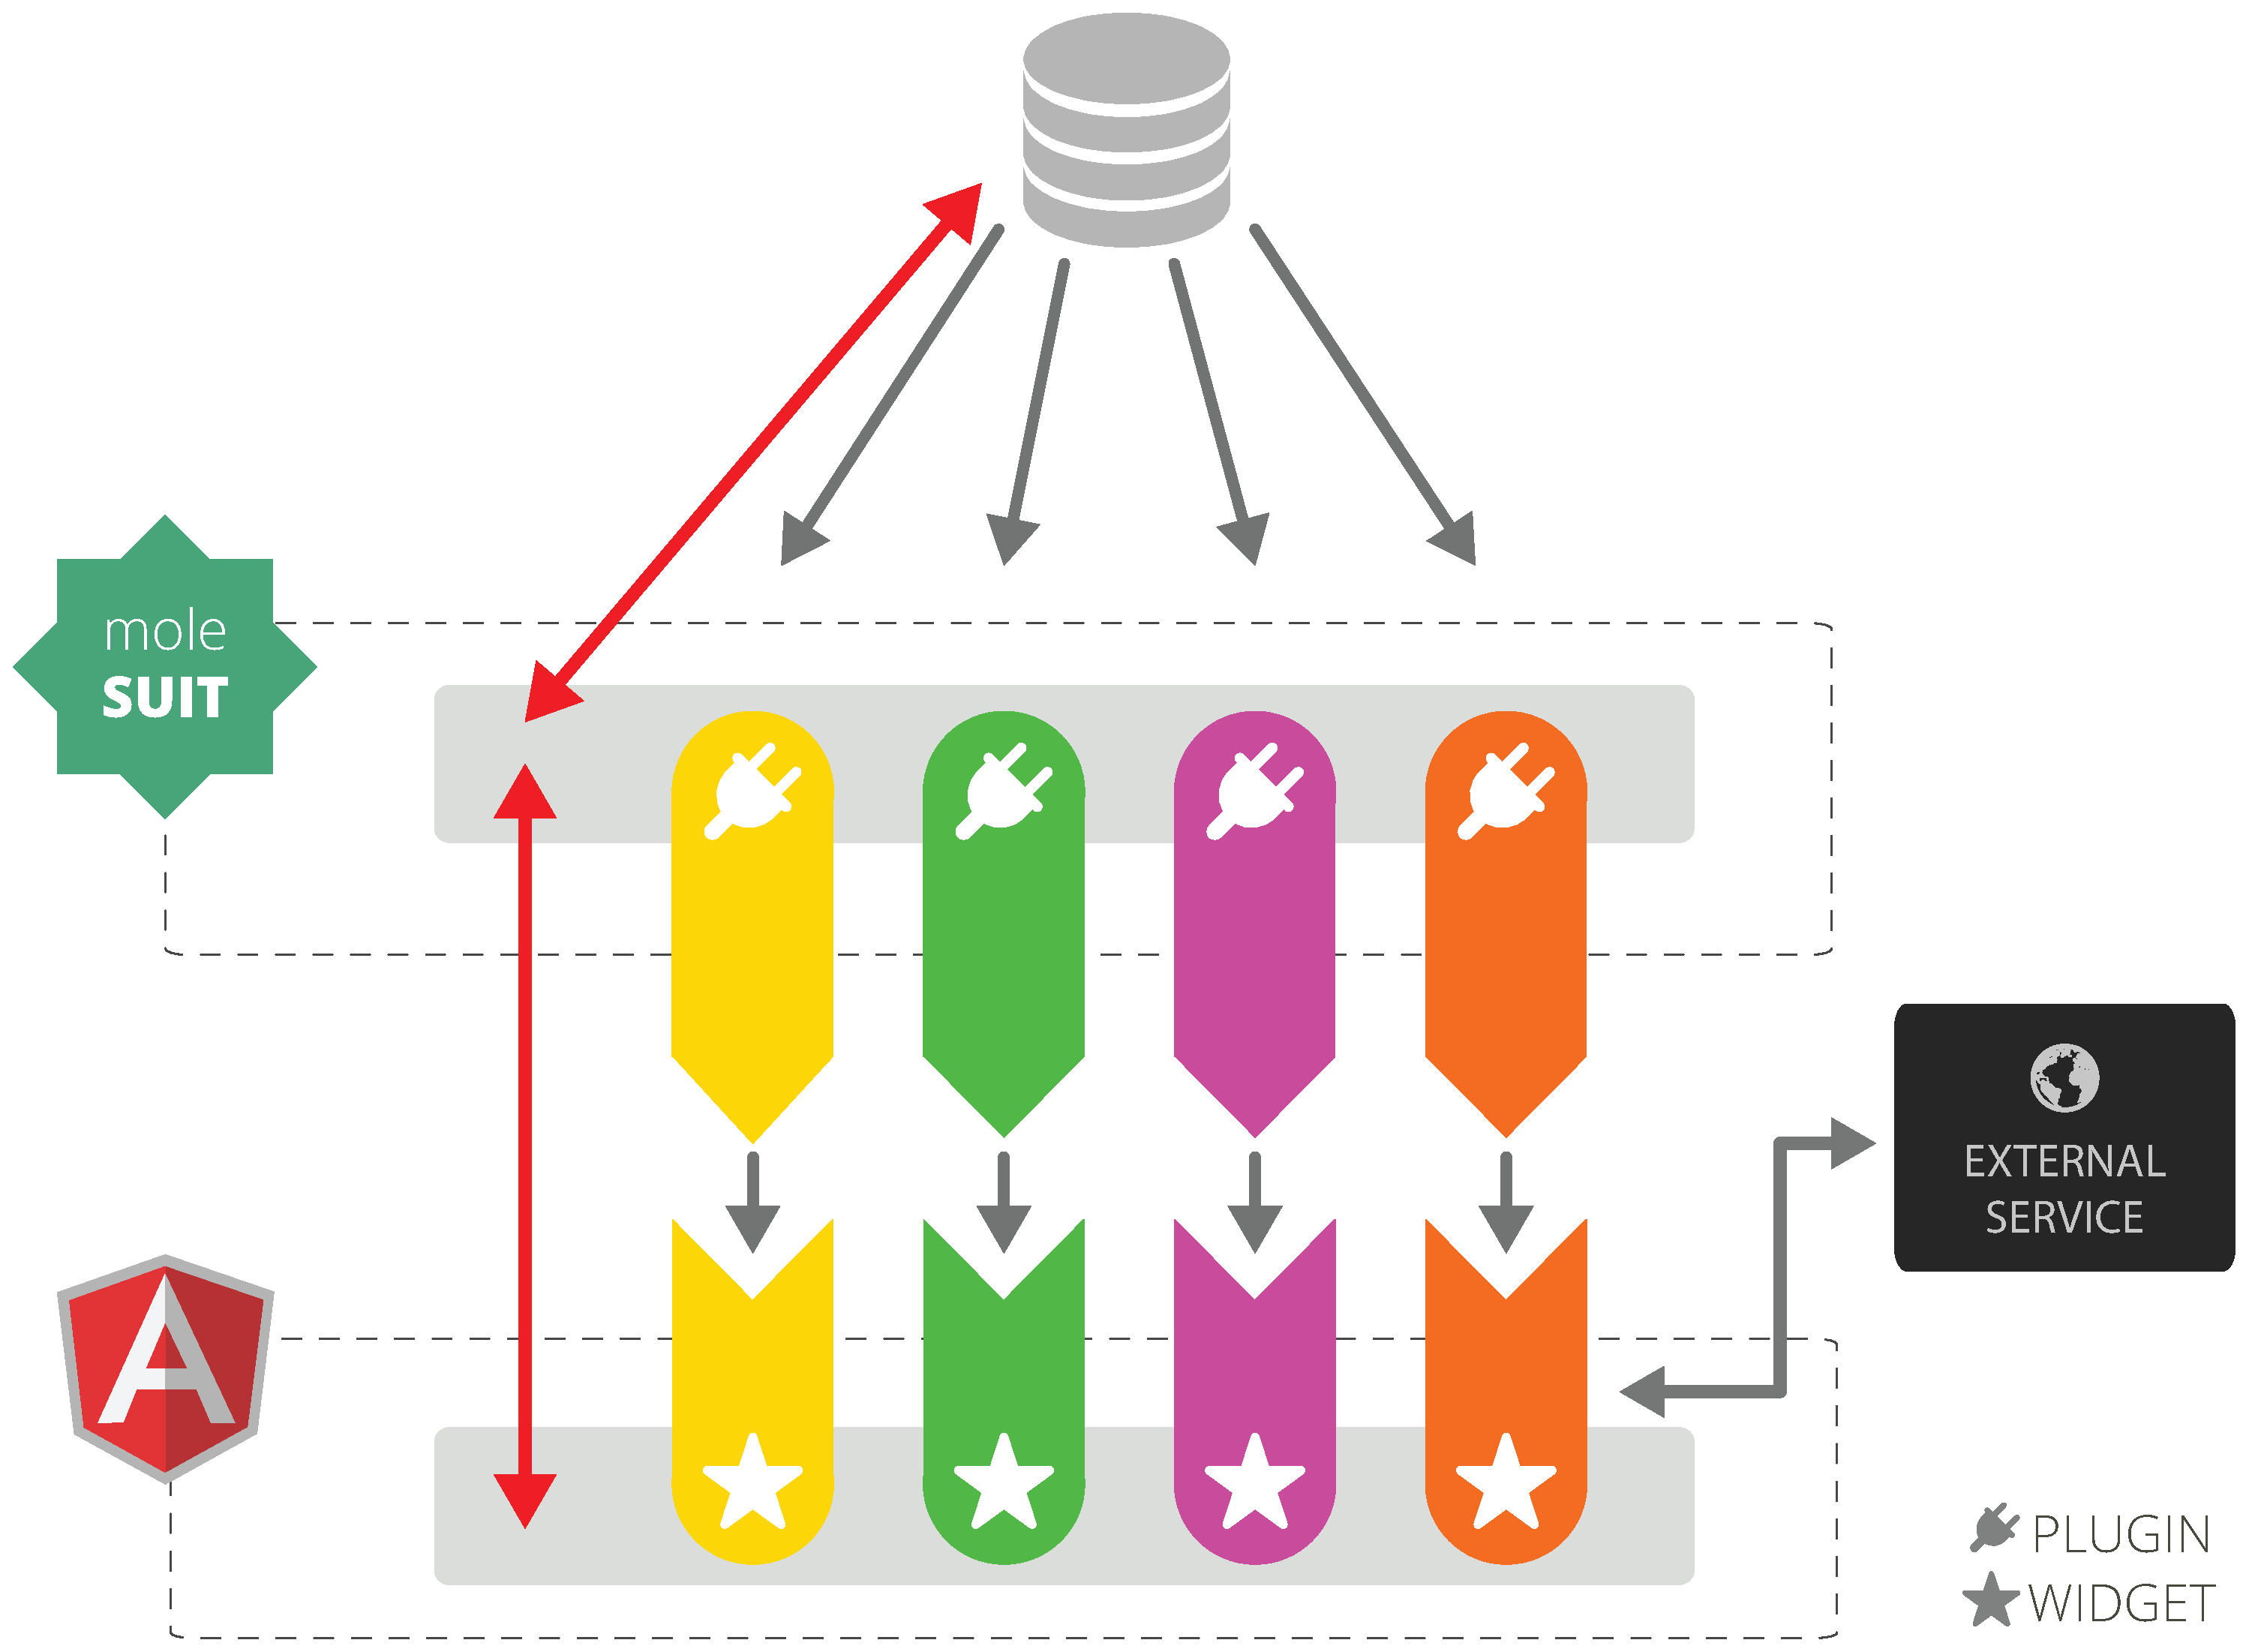
\includegraphics[width=1.0\linewidth]{./img/mole-suit}
\caption[Architettura di mole-suit]{Architettura di mole-suit}
\label{fig:mole-suit}
\end{figure}

La figura \ref{fig:mole-suit} fornisce una rappresentazione schematica delle componenti di Mole Suit. 

Gli utilizzatori accedono al sistema attraverso l'interfaccia utente AngularJS. La UI � composta da widget che hanno il compito di interrogare i rispettivi plugin, residenti nel server mole-suit, al fine di estrarre i dati necessari al popolamento delle pagine web richieste.


al fine di ottenere i dati necessari al popolamento delle pagine web richieste.

 


Il server mole-suit si interfaccia con il database ed estrae i dati denormalizzati. Le informazioni ottenute vengono quindi

li invia alla User Interface (UI) AngularJS che si occupa della vera e propria costruzione della pagina web all'interno del browser dell'utente.

\subsubsection{I Plugin}



\subsubsection{La User Interface}

L'interfaccia utente di Mole.io � interamente realizzata utilizzando AngularJS, descritto in \ref{AngularJS_e_altre_tecnologie_di_frontend}. Questa tecnologia permette di implementare applicazioni web in grado di essere eseguite completamente client-side. 

La costruzione delle pagine HTML da mostrare all'utente �, quindi, a carico del computer dell'utente stesso, non del server che fornisce l'applicazione. Ogni client ha, ovviamente, la necessit� di comunicare con il server, al fine di ottenere i dati per popolare le pagine da mostrare all'utente. 

Questo approccio permette di minimizzare la quantit� di informazioni inviate dal server al client con il conseguente aumento delle performance dell'applicazione stessa.

In gergo tecnico, le applicazioni realizzate con AngularJS, si definiscono \textit{servibili staticamente}. Questo termine sottolinea il fatto che non esiste la necessit� di costruire pagine lato server e, di conseguenza, � possibile utilizzare server minimali, molto economici in termini di risorse di sistema, per fornire questo tipo di applicazioni.

% l'idea � stata costruire un sistema di widget usando de directive angular

\subsubsection{Gli Widget}



\subsubsection{Il Workflow con Mole.io}

Al primo accesso Mole.io, mostra la \textit{homepage} pubblica dell'applicazione. Questa pagina riporta un messaggio di benvenuto ed un bottone, con il quale � possibile procedere all'autenticazione con Twitter, utilizzando il protocollo OAuth 2.0, come descritto in \ref{Autenticazione_degli_utenti}.

Una volta eseguita la procedura di accesso, si raggiunge una pagina \textit{Getting Started}, nella quale � descritta la sequenza delle operazioni necessarie per utilizzare Mole.io. L'immagine \ref{fig:workflow-auth} riporta le schermate proposte dal sistema durante le operazioni descritte.\\

\begin{figure}[h]
\centering
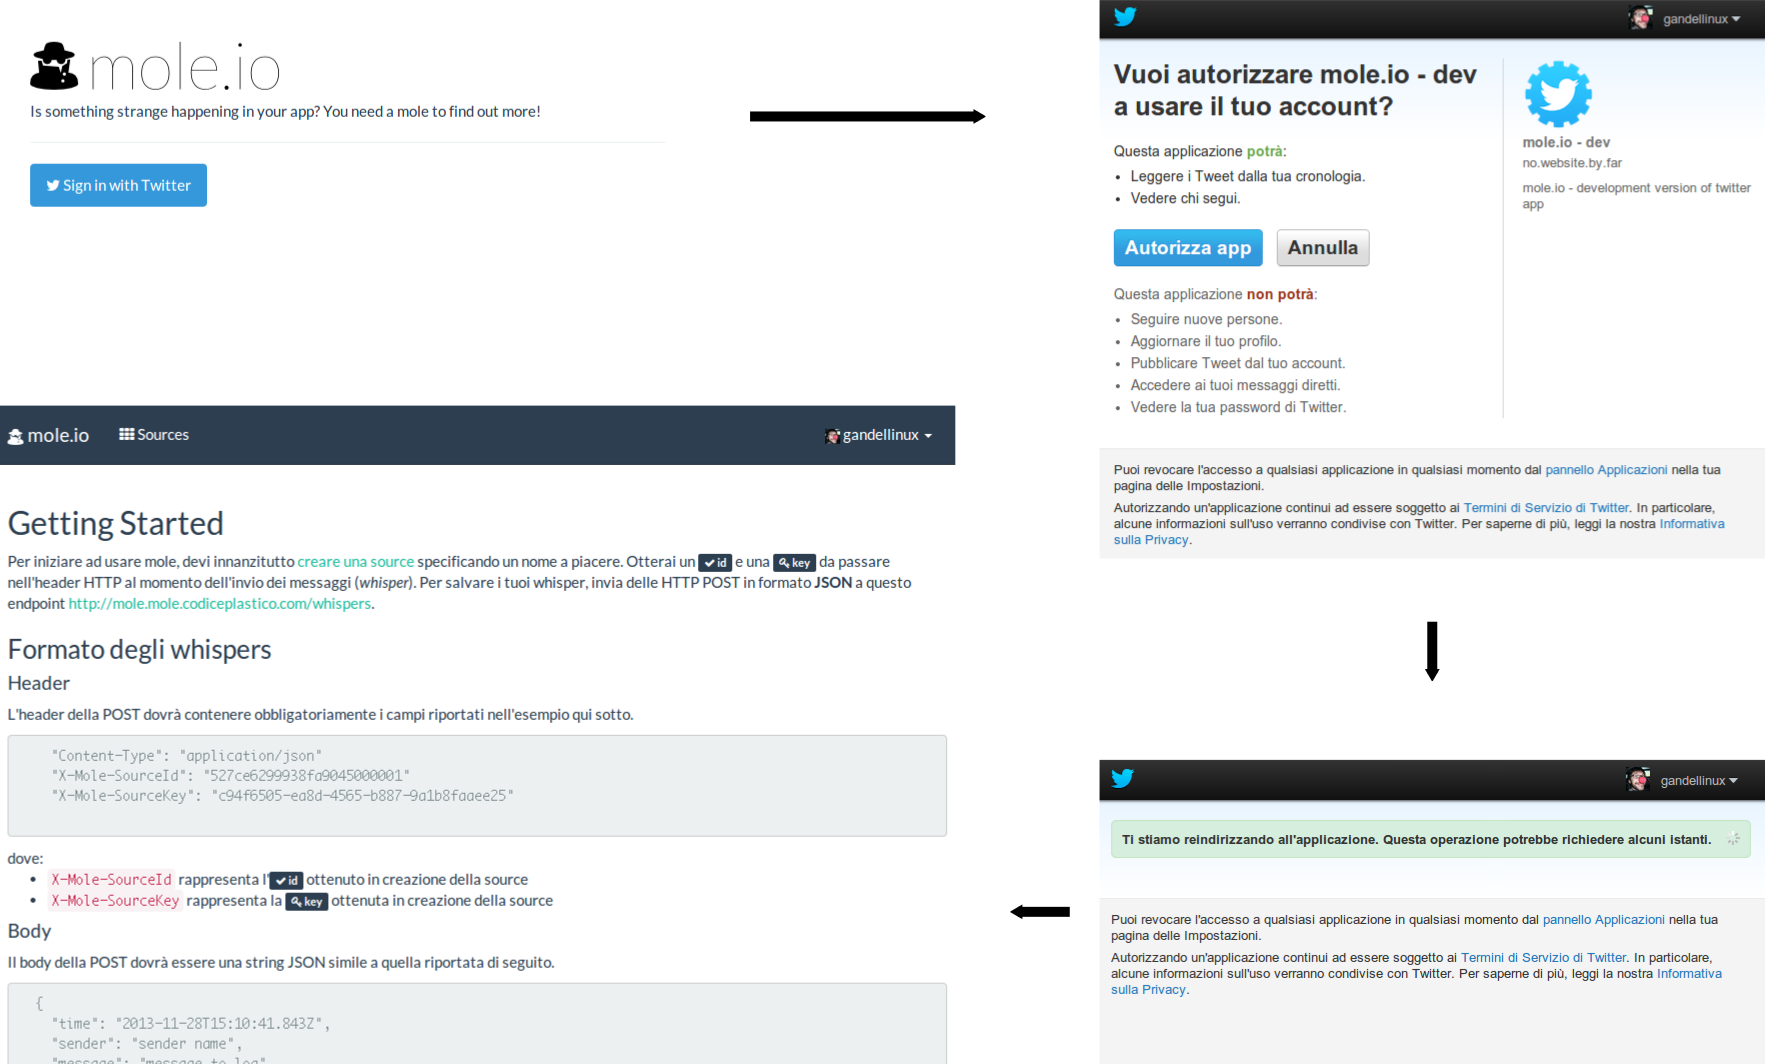
\includegraphics[width=1.0\linewidth]{./img/workflow-auth}
\caption[Accesso a Mole.io]{Accesso a Mole.io}
\label{fig:workflow-auth}
\end{figure}

Cliccando sulla voce \textit{Sources}, nella barra superiore dell'applicazione, � possibile accedere alla pagina per la creazione e visualizzazione delle sources: le applicazioni da monitorare. Per aggiungere una nuova source � sufficiente inserire il nome desiderato nell'apposito campo di testo e premere il pulsante con il simbolo \textquotedblleft+\textquotedblright. L'immagine \ref{fig:workflow-sources} mostra le fasi di questa procedura.

\begin{figure}[h]
\centering
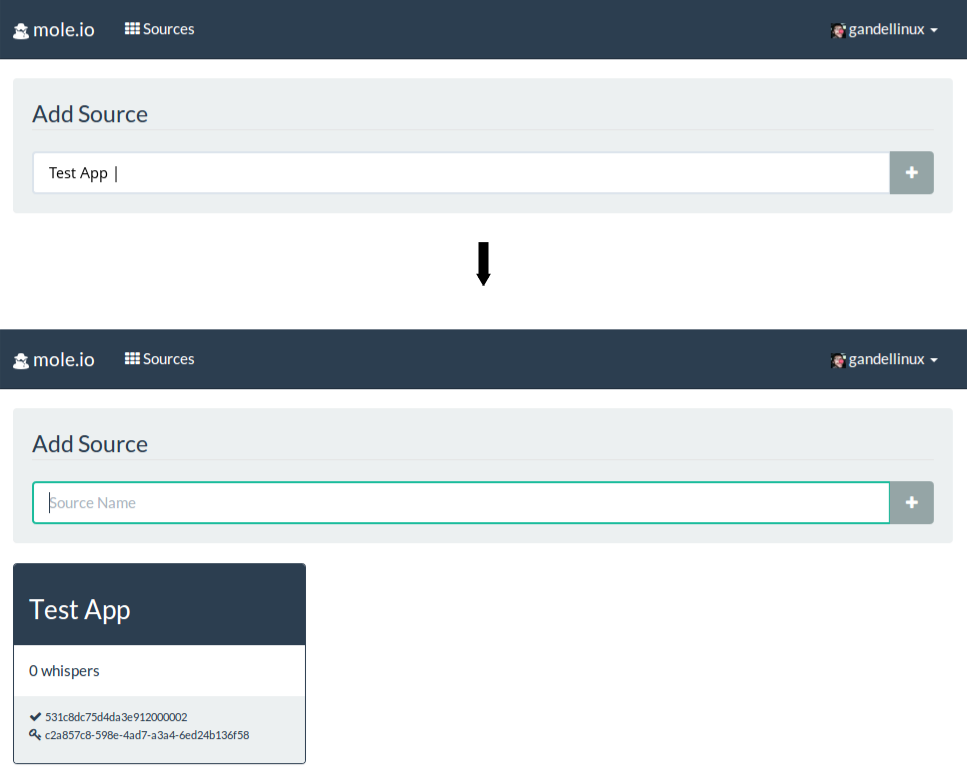
\includegraphics[width=1.0\linewidth]{./img/workflow-sources}
\caption[Creazione di una Source]{Creazione di una Source}
\label{fig:workflow-sources}
\end{figure}

Una volta creata la source, Mole.io restituisce due codici associati ad essa: un \verb|id| e una \verb|key|. Questi dati dovranno essere utilizzati per configurare il mole-contact presente all'interno dell'applicazione da monitorare, e permetteranno al server mole di identificare la provenienza dei messaggi inviati da tale applicazione.




% plugin <--> widget
% c'� anche una comunicazione diretta tra ui e server, per il recupero di informazioni di base, non denormalizzate







% pezzi

% architettura della 

% spiegare un workflow "tipo" per 
% x iscrizione/login
% x creazione di una source
% - attesa dei dati
% - visualizzazione delle info

% screenshot della UI (durante la spiega del flow)

% dire che la ui � separata e statica e pu� essere servita da un terzo server

% come funziona la storia id/key per autenticarsi sulle api

% come scrivere plugin e widget?

